\subsubsection{MVC pattern}

    Our system will be strongly based on the MVC architectural pattern; this choice is due to the fact that this pattern will help us reducing the complexity of the structure of the system, by distributing all the functionalities between three interconnected parts (model, view and controller).
    \newline
    \newline
    The following schema explains this pattern:
    \begin{figure}[H]
            \centering
            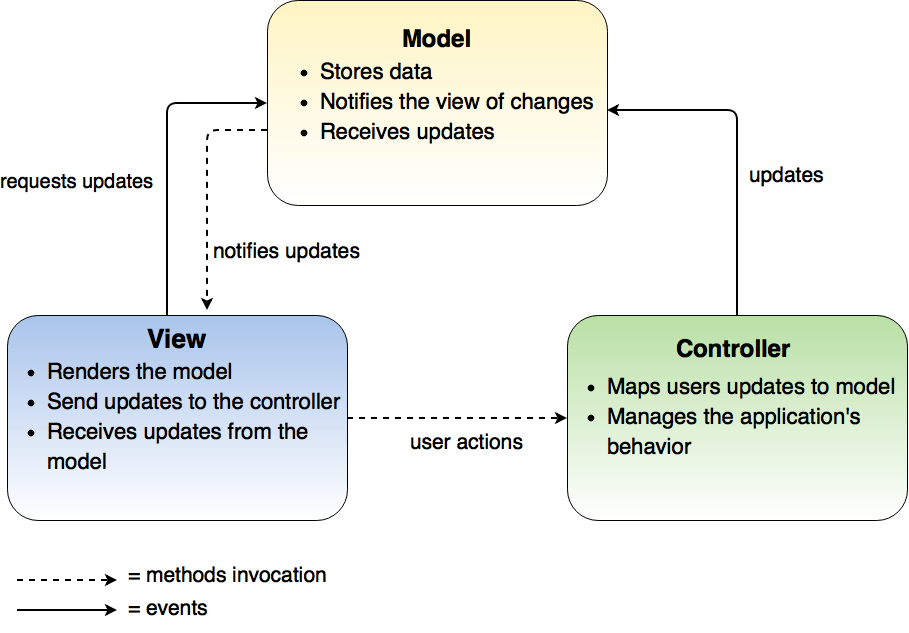
\includegraphics[width=14cm]{./Images/MVC.png}
            \caption{MVC pattern}
    \end{figure}

\subsubsection{State pattern}

    This pattern will be used to manage the behaviour of the taxi drivers; indeed, taxi drivers will be provided with a status (that can be 'AVAILABLE', 'NOTAVAILABLE' or 'OFFLINE' as discussed in the RASD\footnote{\label{note1}see the Class Diagram in the 'Specific Requirements' section}) and, according to their state, they will be able to perform only some specific actions.
    For example, if the status of a taxi driver is 'NOTAVAILABLE', he will not be inserted in any queue and so he will be not allowed to accept any request.
    \newline
    Further, this pattern will be used also for request; each request has a status (that can be 'WAITING', 'RIDING', 'COMPLETED' as discussed in the RASD\footnotemark[\ref{note1}]) and also in this case, according to the status of the request, only some specific kind of actions can be performed. For instance, if the status of a request is 'RIDING', it means that there must be a taxi driver associated to that request, while if a request is 'WAITING' there are no taxi drivers associated to this request.
    
\subsubsection{Client-server model}

    In our project, we have referred to this model two times: for the communication between the clients and the web server and the one between the application server and the database.
    
\subsubsection{REST}
    
    The mobile applications on the front-end of the system will communicate with the application server thanks to a RESTful interface that is implemented on the application server. So, the mobile device will send requests using the HTTPS protocol and then it will receive from the application server JSON data that it will parse to extract information.
    \newline
    We have preferred REST to SOAP because a RESTful interface is easier to implement, while SOAP requires a more rigid and complex structure. Further, SOAP returns XML data that are more difficult to parse than JSON messages, which on the contrary are concise and not so verbose. This last consideration was a very important point for our choice: we want to avoid that our mobile application will be too heavy and so we have preferred the REST+JSON structure.
    
\subsubsection{Web services}
    
    Our system is also provided with a web service that is offered in the mobile application of taxi drivers. Once a taxi driver have accepted a request, the application will give geolocation information about the journey he has to take care of. Moreover, this service will provide the average time a passenger has to wait for the taxi arrival and also the average time the taxi will take to reach the destination.
    \newline
    In order to do so, we have decided to use an external service, Google Maps, and our choice is due to different reasons: first of all, we have decided not to implement this service manually because it would be so difficult and secondly, Google Maps is a very powerful and well-known software, that almost everybody is able to use.
    \newline
    Google Maps API provide interfaces to Google Maps services and allow to request data that can be used in our application; in our case, this means that our mobile application will send HTTP requests to a specific URL (according to the specific service we need), passing some parameters; then, the service will return JSON data that will be parsed by the application in order to get some geolocation data or distance values.